% Author         : Pedro Ferreira (up201806093@up.pt)
% Version        : 1.0
% Created on     : 12.08.2022
% Last Edited on : 14.08.2022

% Adapted from HSRM theme by Benjamin Weiss
% Copyright      : Copyright (c) 2013-2014 by Benjamin Weiss. All rights reserved.
% License        : This file may be distributed and/or modified under the
%                  GNU Public License.
% Description    : HSRM beamer theme demonstration. Also includes a short 
%                  Tutorial regarding the beamer class.



%%%%%%%%%%%%%%%%%%%%%%%%%%%%%%%%%%%%%%%%%%%%%%%%%%%%%%%%%%%%%%%%%%%%%%%%%%%
%                    !!! Compile with LuaLaTex !!!
%%%%%%%%%%%%%%%%%%%%%%%%%%%%%%%%%%%%%%%%%%%%%%%%%%%%%%%%%%%%%%%%%%%%%%%%%%%

\documentclass[compress,aspectratio=169]{beamer}
%--------------------------------------------------------------------------
% Common packages
%--------------------------------------------------------------------------
\usepackage[british]{babel}
\hypersetup{
pdftitle={Sleek Beamer Theme},
pdfsubject={Latex},
pdfauthor={Pedro Paulo Carneiro Ferreira},
pdfkeywords={Latex,Beamer}}

\usepackage{graphicx}
\usepackage{multicol}
\usepackage{wrapfig}
\usepackage{caption}
\newcommand*{\captionsource}[2]{%
  \caption[{#1}]{%
    #1%
    \\\hspace{\linewidth}%
    \textbf{Source:} #2%
  }%
}
\newcommand{\backupbegin}{
   \newcounter{finalframe}
   \setcounter{finalframe}{\value{framenumber}}
}
\newcommand{\backupend}{
   \setcounter{framenumber}{\value{finalframe}}
}
\usepackage{float}

% Advanced table functions
\usepackage{tabularx,ragged2e}
\usepackage{booktabs}
% Listings extension
\usepackage{listings}

%--------------------------------------------------------------------------
% Load theme
%--------------------------------------------------------------------------
\usepackage{sleektheme/beamerthemesleek}
\usetheme[]{sleek}

\usepackage{sleektheme/dtklogos} % must be loaded after theme
\usepackage{tikz}
\usetikzlibrary{mindmap,backgrounds}

\usepackage[
    backend=biber,
    style=numeric,
    sorting=none
]{biblatex}
\addbibresource{bibliography.bib}

%--------------------------------------------------------------------------
% General presentation settings
%--------------------------------------------------------------------------
\title{The Influence of Cyclists\\ on Traffic }
\subtitle{ }
\date{19th December 2022}
\author{Nils Egger, Sophia Herrmann, Jan Hochstrasser,\\ Jannick Schröer, Alexander Sotoudeh}
\institute{ETH Zürich\\ {\Medium Complex Social Systems: Modeling Agents, Learning, and Games}}

%--------------------------------------------------------------------------
% Notes settings
%--------------------------------------------------------------------------
\setbeameroption{show notes}

\begin{document}
%--------------------------------------------------------------------------
% Titlepage
%--------------------------------------------------------------------------

\maketitle

%\begin{frame}[plain]
%	\titlepage
%\end{frame}

%--------------------------------------------------------------------------
% Table of contents
%--------------------------------------------------------------------------
\section*{Structure}
\begin{frame}{Structure}
	% hideallsubsections is recommended for longer presentations
	\tableofcontents[hideallsubsections]
\end{frame}

%--------------------------------------------------------------------------
% Content
%--------------------------------------------------------------------------

\section{Motivation}

\subsection{Motivations}
\begin{frame}[containsverbatim, fragile]{Motivation}
Traffic jams and congestions lead to many unfavorable effects:
\begin{itemize}
	\item<2->[-] Pollution
	\item<3->[-] Health Hazards
	\item<4->[-] Tangible Costs
\end{itemize}
\end{frame}

% \begin{frame}[containsverbatim, fragile]{Motivation}

% \begin{itemize}
% 	\item Pollution
% 	\item Health Hazards
% 	\item Tangible Costs
% \end{itemize}
% \end{frame}

\begin{frame}[containsverbatim, fragile]{Health Hazards}
Higher traffic volume results in higher levels of nitrogen dioxide, in an almost linear relation. \cite{zhang} Higher $NO_2$ results in
\begin{itemize}
	\item<2->[-] Increased respiratory diseases \cite{goudarzia}
	\item<3->[-] Heart issues \cite{goudarzia}
\end{itemize}
\end{frame}

\begin{frame}[containsverbatim, fragile]{Tangible Cost}
Congestions and traffic jams leads to a cost, which is measured by three factors:
\begin{itemize}
	\item<2->[-] accidents and collisions
        \begin{itemize}
            \item<3->[-] 210.2 billions euros of damages per year in EU \cite{eurocomm}
        \end{itemize}
	\item<4->[-] environmental impact
        \begin{itemize}
            \item<5->[-] 21.3 euros on average per kilogram of $NO_2$ \cite{swissno2}
            \item<6->[-] 35 781 tonnes in 2015 in CH \cite{swissno2}
        \end{itemize}
        \item<7->[-] scarcity cost
        \begin{itemize}
            \item<8->[-] 208.3 billion euros in EU \cite{eurocomm}
        \end{itemize}
\end{itemize}
\end{frame}




\begin{frame}[containsverbatim, fragile]{Corona Surge}
Bicycling saw a huge surge in popularity post Covid-19. 
	\begin{figure}
		\centering
		\includegraphicscopyright[width=0.8\textwidth]{Images/CoronaBikes.png}
{Source:  \href{https://ivtmobis.ethz.ch/mobis/covid19/reports/latest_de#MOBIS-COVID19}{MOBIS-COVID19}}
	\end{figure}
\end{frame}



\begin{frame}[containsverbatim, fragile]{Velostrategie 2030}
	\begin{multicols}{2}
        Zurich itself is pushing for more environment friendly modes of transportation. 
        \vspace{-1cm}
            \begin{itemize}
            \setlength\itemsep{4mm}
        	\item<2->[-] currently around 10\% bicycles \cite{bericht21}
        	\item<3->[-] goal is to increase by 10 percent points \cite{velo2030}
            \item<4->[-] how does this affect traffic?
		\end{itemize}
        \columnbreak
        \begin{figure}
		\includegraphicscopyright[height=0.35\textwidth]{Images/Velostrategie2030.png}{Source: \href{https://www.stadt-zuerich.ch/content/dam/stzh/site/velo/4_die-strategien/Velostrategie\%202030.pdf}{Stadt Zürich}}
	\end{figure}
	\end{multicols}
\end{frame}


\subsection{Question}
\subsection{Relevance}
\subsection{Similar Projects}

\section{Model}
\subsection{Environment}
\begin{frame}[containsverbatim, fragile]{Open Street Map}

\only<2>{
        \begin{wrapfigure}[16]{r}{0.375\textwidth}
        \centering
            \vspace{-0.4cm}
            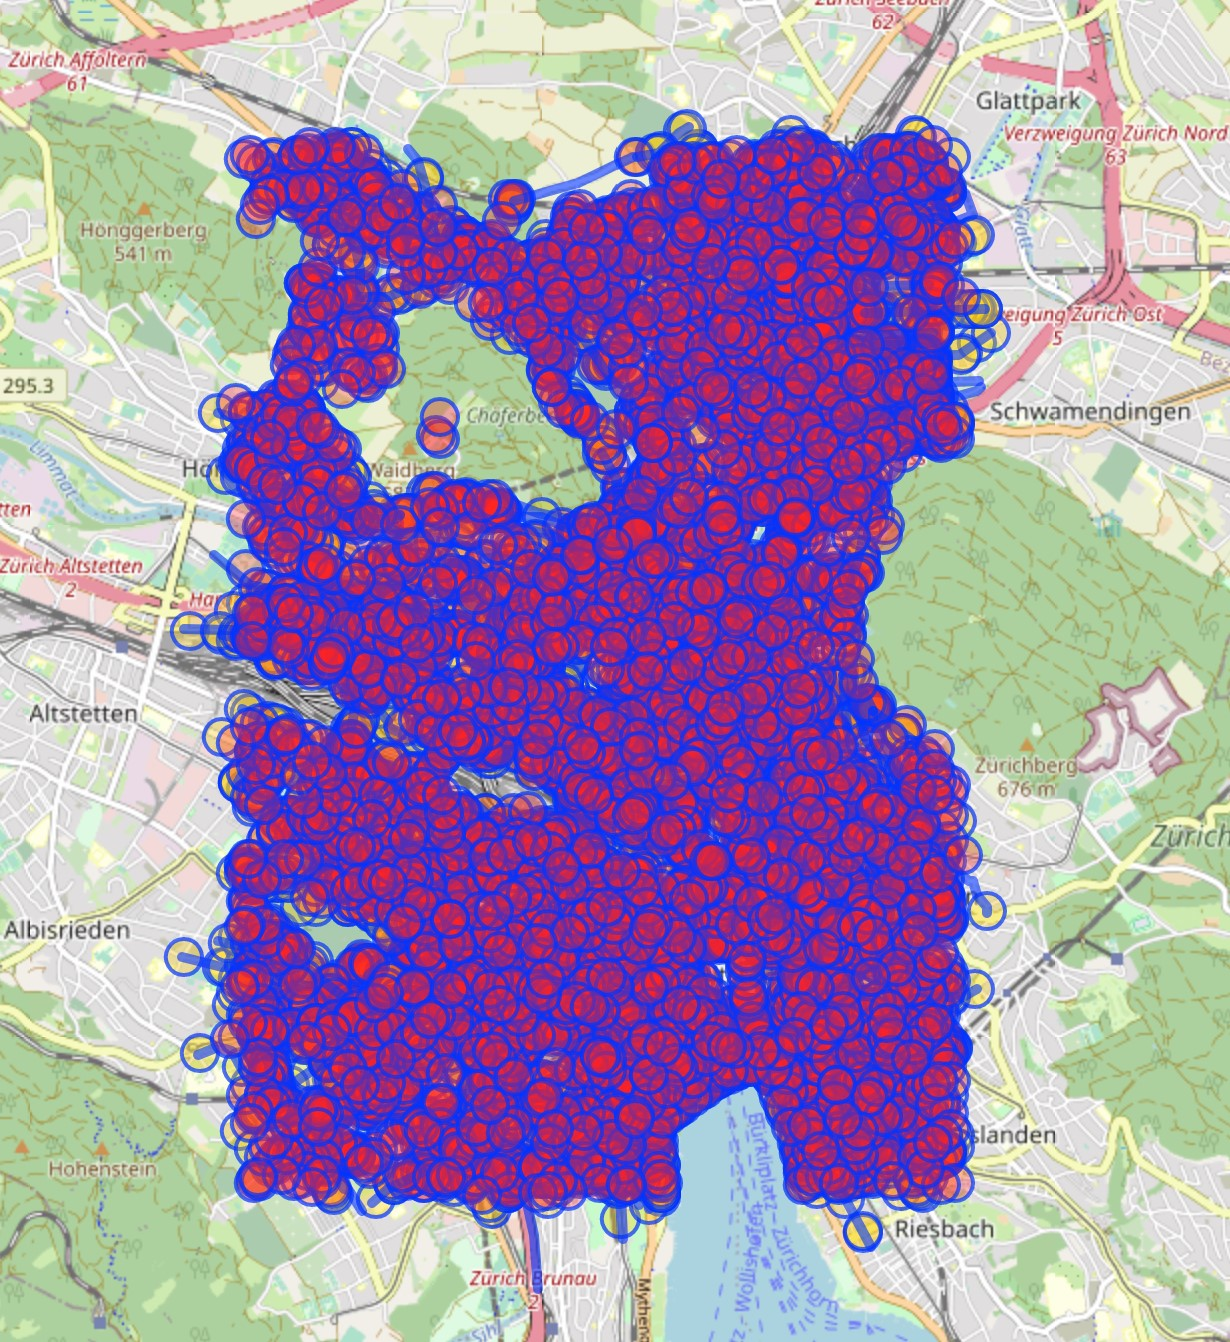
\includegraphics[width=\linewidth]{./Images/road-network.jpeg}
            %\captionsource{Modelled Road Network}{Screenshot taken from Overpass Turbo}\label{network}
        \end{wrapfigure}
 }
 
\begin{lstlisting}[breakindent=0pt, tabsize=1]
[out:json]
[bbox:47.36, 8.50, 47.42, 8.56];
    (
        way[highway=primary];
        way[highway=secondary];
        way[highway=trunk];
        way[highway=tertiary];
        way[highway=service];
        way[highway=residential];
    )->.a;
    (.a;>;);
out;
\end{lstlisting}

\end{frame}


\begin{frame}[containsverbatim, fragile]{Environment}
\only<1->{
    \only<1>{\vspace{-2.4cm}}
    \only<2-5>{\vspace{-1.25cm}}
        Streets and Intersections make up the Model Environment. 
	\begin{multicols}{2}
        \mbox{}
        \only<2->{
        Intersections are characterized by:
        \only<6->{\vspace{-1.8cm}}
            \begin{itemize}
            \setlength\itemsep{1mm}
        	\item<3->[-] IDs
        	\item<4->[-] coordinates
            \item<5->[-] incident streets
		\end{itemize}
        }
        \columnbreak
        \mbox{}
        \only<6->{
         Streets are characterized by:
             \begin{itemize}
                \item<7->[-] ID
         	\item<8->[-] start/end crossing IDs
                \item<9->[-] lanes
                \item<10->[-] length 
                \item<11->[-] speed limit
                \item<12->[-] if present: opposite street ID
		 \end{itemize}
        }
	\end{multicols}
 }
\end{frame}

\subsection{Agents}
\begin{frame}[containsverbatim, fragile]{Agents}

        \begin{wrapfigure}[10]{r}{0.3\textwidth}
        \centering
            \vspace{-0.5cm}
            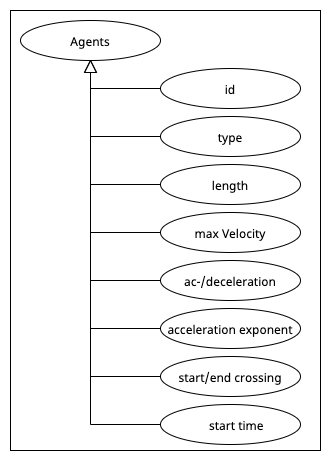
\includegraphics[width=\linewidth]{./Images/Agents.png}
        \end{wrapfigure} 
        
        Agents can be of one of two types, bicycles or cars. Both share the same attribute types but they are chosen out of different intervals.

        \begin{table}[H]
\hspace{-4.5cm}
\begin{tabularx}{0.85\linewidth}{C|C|C}
    \textbf{Attribute} & \textbf{Car} & \textbf{Bike}\\
    \hline
    \textbf{Length} $(m)$ & $[3.5, 5]$ & $[1.5, 2.5]$\\
    \hline
    \textbf{ Max. Velocity} $(km/h)$ & $[100, 250]$ & $[10, 35]$\\
    \hline 
    \textbf {Acceleration} $(m/s^2)$ & $[1.5, 5]$ & $[0.5, 1.5]$\\
    \hline
    \textbf{Deceleration} $(m/s^2)$ & $[2,6]$ & $[1,3]$ \\
    \hline
    \textbf{Acceleration Exponent} & $[8, 12]$ & $[8,12]$
\end{tabularx}
\end{table}

\end{frame}


\subsection{Interaction}
\begin{frame}[containsverbatim, fragile]{Vehicles Behaviour}
	%insert flow chart that describes interactions here
        \begin{figure}
		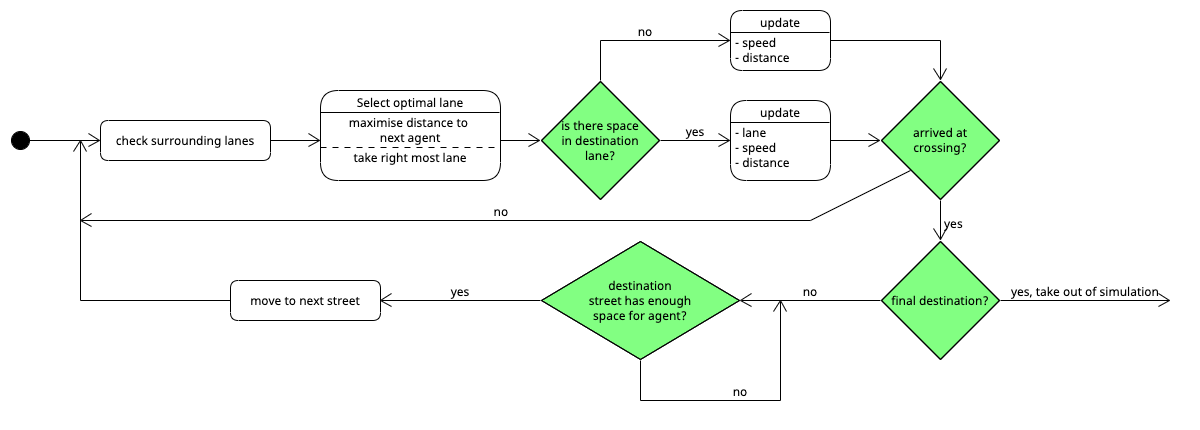
\includegraphics[width=1\textwidth]{Images/AgentBehaviour.png}
	\end{figure}
\end{frame}

\begin{frame}[containsverbatim, fragile]{Differences between Cars and Bikes}
\vspace{-1cm}
        \begin{multicols}{2}
        Bicycles:
        \begin{itemize}
        \setlength\itemsep{1mm}
            \item<2->[-] Bicycles can be on streets and bicycle lanes
            \item<3->[-] Bikes are smaller $\rightarrow$ higher density is possible
            \item<4->[-] Bikes have lower max speeds and acceleration
        \end{itemize}
       
        \columnbreak
        \mbox{}
        \only<4->{
        Cars:
        \vspace{-0.1cm}
            \begin{itemize}
            \setlength\itemsep{1mm}
        	   \item<5->[-] Cars can only be on streets
        	   \item<6->[-] Cars are larger 
                  \item<7->[-] Cars accelerate faster and have a higher max speed
		\end{itemize}
        }
	\end{multicols}
\end{frame}


\section{Results}
\begin{frame}[containsverbatim, fragile]{Average Speed}
        \vspace{-0.2cm}
        \begin{figure}
		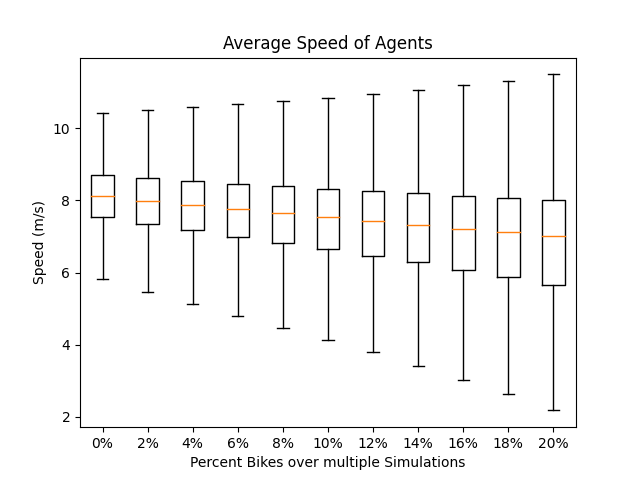
\includegraphics[width=0.65\textwidth]{Images/avg_speed_agent.png}
	\end{figure}
\end{frame}

\begin{frame}[containsverbatim, fragile]{Traffic Flow}
\vspace{-0.2cm}
        \begin{figure}
		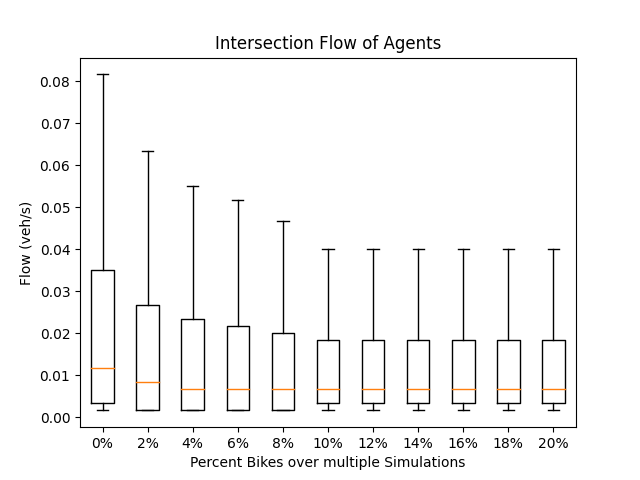
\includegraphics[width=0.65\textwidth]{Images/intersection_flow_agent.png}
	\end{figure}
\end{frame}

\begin{frame}[containsverbatim, fragile]{Traffic Density}
\vspace{-0.2cm}
        \begin{figure}
		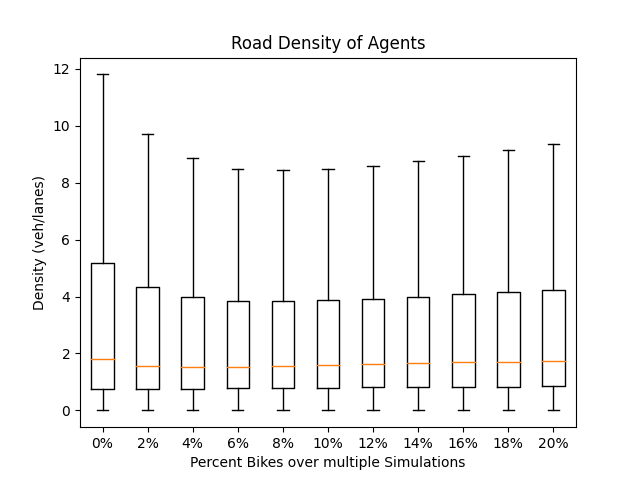
\includegraphics[width=0.65\textwidth]{Images/road_density_agent.png}
	\end{figure}
\end{frame}
\section{Outlook}

\begin{frame}[containsverbatim, fragile]{Abstractions}
\begin{itemize}
    \item<2->[-] Model only considers cars and bikes, no public transport or other vehicles
    \item<3->[-] Couldn't find proper travel data
    \begin{itemize}
        \item<4->[-] Start and end points are randomized
        \item<5->[-] Amount of agents is evenly distributed over the simulation
    \end{itemize}
    \item<6->[-] Cutoff point for streets was chosen slightly higher than real world counterpart
    \item<7->[-] Model doesn't incorporate driving styles, lawfulness
    \item<8->[-] No consideration for extraordinary events: Accidents, Road Construction
\end{itemize}
\end{frame}

\begin{frame}[containsverbatim, fragile]{Conclusion}
\begin{itemize}
    \item<2->[-] no big effect on average speed, density or flow
    \item<3->[-] no significant change in density
    \begin{itemize}
        \item<4->[-] no congestion relief
        \item<5->[-] no negative impact either
    \end{itemize}
    \item<6->[-] other reasons for changing to bicycles
    \begin{itemize}
        \item<7->[-] less environmental pollution
        \item<8->[-] quieter city
    \end{itemize}
\end{itemize}
\end{frame}

\begin{frame}[containsverbatim, fragile]{Further Extensions}
In a continuation of this project, things that could be of interest to study could be:
\begin{itemize}
    \item<2->[-] Including public transport, pedestrians, etc.
    \item<3->[-] Seasons, as bicycle usage is weather dependant
    \item<4->[-] More realistic routes and agent amount
    \item<5->[-] Larger road network
    \item<6->[-] Higher complexity for agent behavior, overtaking on opposite roads etc.
    \item<7->[-] Calculating the associated cost difference
\end{itemize}
\end{frame}


%\section{Live Demo}

\section{Q\&A}

\begin{frame}[containsverbatim, fragile]{References}
\printbibliography
\end{frame}

\appendix
\begin{frame}[containsverbatim, fragile]
\vspace{-0.2cm}
        \begin{figure}
		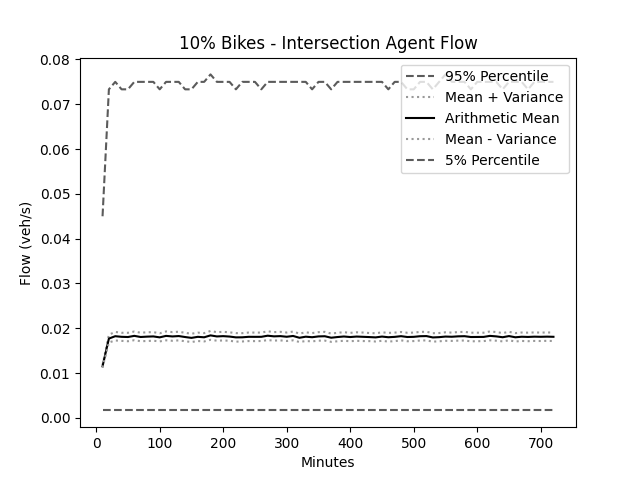
\includegraphics[width=0.65\textwidth]{Images/intersection_agent_flow.png}
	\end{figure}
\end{frame}

\begin{frame}[containsverbatim, fragile]
\vspace{-0.2cm}
        \begin{figure}
		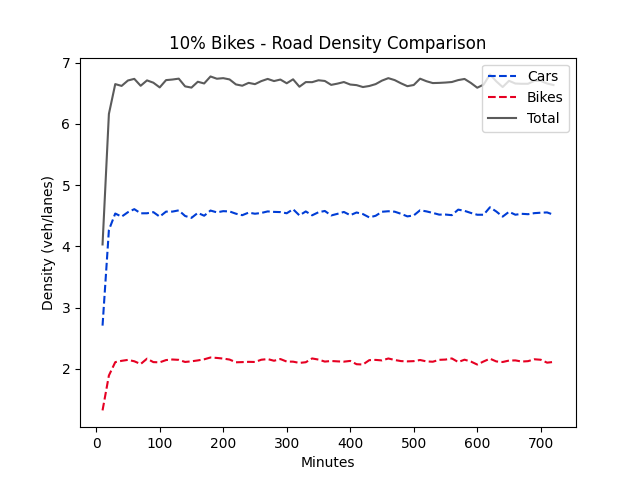
\includegraphics[width=0.7\textwidth]{Images/road_density_comparison.png}
	\end{figure}
\end{frame}

\begin{frame}[containsverbatim, fragile]
\vspace{-0.2cm}
        \begin{figure}
		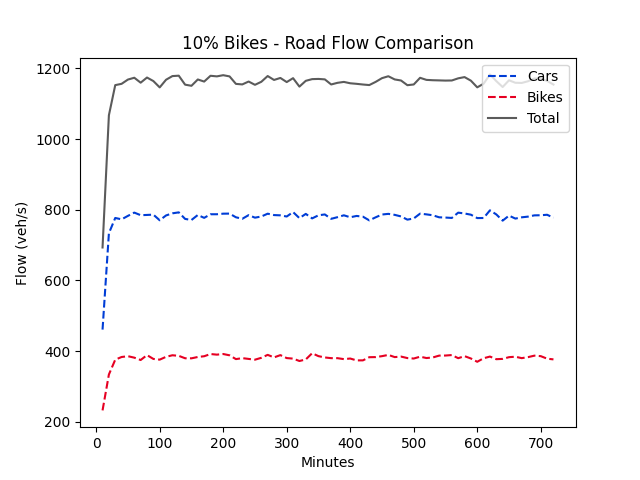
\includegraphics[width=0.7\textwidth]{Images/road_flow_comparison.png}
	\end{figure}
\end{frame}

\begin{frame}[containsverbatim, fragile]
\vspace{-0.2cm}
        \begin{figure}
		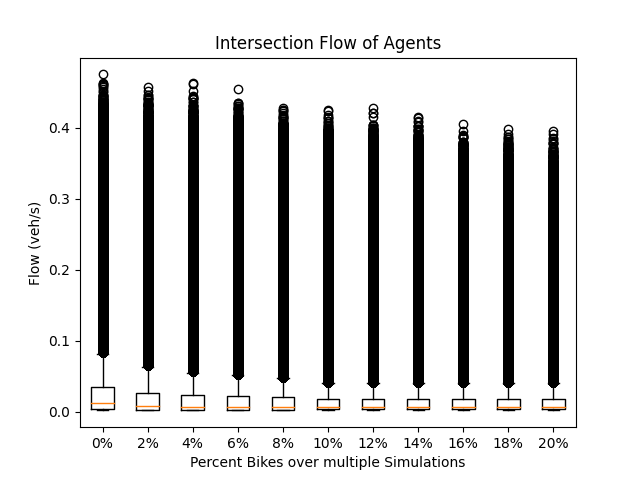
\includegraphics[width=0.7\textwidth]{Images/intersection_flow_agent(Fliers).png}
	\end{figure}
\end{frame}
% AB HIER NUR NOCH TEMPLATE






% \section{Introduction}

% \begin{frame}{What is Beamer?}
% 	The beamer classes for \LaTeX\ are used to create presentations that are to be shown with a beamer. The text typesetting system creates PDF files that can be shown by a large number of programmes.
	
% 	The present theme was adapetd from HSRM theme by Benjamin Weiss and it makes the creation of slides (assuming basic knowledge of \LaTeX\ ) child's play.
% \end{frame}

% \begin{frame}{System requirements}
% 	In order to successfully create presentations with this theme, the following requirements must be met by the system:
% 	\begin{itemize}
% 		\item LuaLaTeX must be used to typeset the slides.
% 		\item Besides some standard packages, the packages \texttt{beamer}, \texttt{pgf} and \texttt{xcolor} must be installed.
% 		\item The fonts \quoted{Flama-Light}, \quoted{Flama-Book} and \quoted{Flama-Medium} should be installed. Alternative: \quoted{Arial}\\\url{http://www.felicianotypefoundry.com/}
% 	\end{itemize}
% \end{frame}

% \section{Tutorial}
% \begin{frame}[containsverbatim]{Basic structure of the document}
% The basic structure is simple:
% \begin{lstlisting}
% \documentclass[compress]{beamer}
% % Theme
% \usetheme{sleek}
% % General presentation settings 
% \title{Presentation title}
% \subtitle{Subtitle of the presentation}
% \author{Your name}
% \institute{Study area\University {\Medium RheinMain}}
% \begin{document}
% %Slides
% \end{document}
% \end{lstlisting}
% \end{frame}

% \begin{frame}{Theme options}
% To customise the presentation, the following options can be selected.
% \begin{table}[]
% 	\begin{tabularx}{\linewidth}{l>{\raggedright}X}
% 		\toprule
% 		\textbf{Option} & \textbf{Effect} \tabularnewline
% 		\midrule
% 		\texttt{noflama} & If you do not have the Flama font you can switch to the Arial font with this option. \tabularnewline
% 		\texttt{noserifmath} & Formulas are also set sans serif. \tabularnewline
% 		\texttt{nosectionpages} & The section introduction pages will be hidden.\tabularnewline
% 		\bottomrule
% 	\end{tabularx}
% 	\label{tab:options}
% \end{table}
% \end{frame}

% \begin{frame}{Primary colours}									
% All colours predefined are listed below and in the following slide. You may add more using the same code structure as in the \texttt{colors.tex} file.


% \begin{multicols}{2}

% \setbeamercolor{sleekmaincolorDemo}{fg=maincolor,bg=white}
% \begin{beamercolorbox}[wd=\linewidth,ht=2ex,dp=0.7ex]{sleekmaincolorDemo}
% 	\texttt{maincolor}
% \end{beamercolorbox}
% \setbeamercolor{sleekRedDemo}{fg=sleekRed,bg=white}
% \begin{beamercolorbox}[wd=\linewidth,ht=2ex,dp=0.7ex]{sleekRedDemo}
% 	\texttt{sleekRed}
% \end{beamercolorbox}
% \setbeamercolor{sleekRedDarkDemo}{fg=sleekRedDark,bg=white}
% \begin{beamercolorbox}[wd=\linewidth,ht=2ex,dp=0.7ex]{sleekRedDarkDemo}
% 	\texttt{sleekRedDark}
% \end{beamercolorbox}
% \setbeamercolor{sleekWarmGreyDarkDemo}{fg=sleekWarmGreyDark,bg=white}
% \begin{beamercolorbox}[wd=\linewidth,ht=2ex,dp=0.7ex]{sleekWarmGreyDarkDemo}
% 	\texttt{sleekWarmGreyDark}
% \end{beamercolorbox}
% \setbeamercolor{sleekWarmGreyLightDemo}{fg=sleekWarmGreyLight,bg=white}
% \begin{beamercolorbox}[wd=\linewidth,ht=2ex,dp=0.7ex]{sleekWarmGreyLightDemo}
% 	\texttt{sleekWarmGreyLight}
% \end{beamercolorbox}

% \setbeamercolor{sleekmaincolorDemoBg}{fg=white,bg=maincolor}
% \begin{beamercolorbox}[wd=\linewidth,ht=2ex,leftskip=.5ex,dp=0.7ex]{sleekmaincolorDemoBg}
% 	\texttt{maincolor}
% \end{beamercolorbox}
% \setbeamercolor{sleekRedDemoBg}{fg=white,bg=sleekRed}
% \begin{beamercolorbox}[wd=\linewidth,ht=2ex,leftskip=.5ex,dp=0.7ex]{sleekRedDemoBg}
% 	\texttt{sleekRed}
% \end{beamercolorbox}
% \setbeamercolor{sleekRedDarkDemoBg}{fg=white,bg=sleekRedDark}
% \begin{beamercolorbox}[wd=\linewidth,ht=2ex,leftskip=.5ex,dp=0.7ex]{sleekRedDarkDemoBg}
% 	\texttt{sleekRedDark}
% \end{beamercolorbox}
% \setbeamercolor{sleekWarmGreyDarkDemo}{fg=white,bg=sleekWarmGreyDark}
% \begin{beamercolorbox}[wd=\linewidth,ht=2ex,leftskip=.5ex,dp=0.7ex]{sleekWarmGreyDarkDemo}
% 	\texttt{sleekWarmGreyDark}
% \end{beamercolorbox}
% \setbeamercolor{sleekWarmGreyLightDemo}{fg=white,bg=sleekWarmGreyLight}
% \begin{beamercolorbox}[wd=\linewidth,ht=2ex,leftskip=.5ex,dp=0.7ex]{sleekWarmGreyLightDemo}
% 	\texttt{sleekWarmGreyLight}
% \end{beamercolorbox}

% \end{multicols}

% \end{frame}

% \begin{frame}{Secondary colours}
% \begin{multicols}{2}

% \setbeamercolor{sleekSec1Demo}{fg=sleekSec1,bg=white}
% \begin{beamercolorbox}[wd=\linewidth,ht=2ex,dp=0.7ex]{sleekSec1Demo}
% 	\texttt{sleekSec1}
% \end{beamercolorbox}
% \setbeamercolor{sleekSec1DarkDemo}{fg=sleekSec1Dark,bg=white}
% \begin{beamercolorbox}[wd=\linewidth,ht=2ex,dp=0.7ex]{sleekSec1DarkDemo}
% 	\texttt{sleekSec1Dark}
% \end{beamercolorbox}
% \setbeamercolor{sleekSec1CompDemo}{fg=sleekSec1Comp,bg=white}
% \begin{beamercolorbox}[wd=\linewidth,ht=2ex,dp=0.7ex]{sleekSec1CompDemo}
% 	\texttt{sleekSec1Comp}
% \end{beamercolorbox}
% \setbeamercolor{sleekSec1CompDarkDemo}{fg=sleekSec1CompDark,bg=white}
% \begin{beamercolorbox}[wd=\linewidth,ht=2ex,dp=0.7ex]{sleekSec1CompDarkDemo}
% 	\texttt{sleekSec1CompDark}
% \end{beamercolorbox}

% \setbeamercolor{sleekSec2Demo}{fg=sleekSec2,bg=white}
% \begin{beamercolorbox}[wd=\linewidth,ht=2ex,dp=0.7ex]{sleekSec2Demo}
% 	\texttt{sleekSec2}
% \end{beamercolorbox}
% \setbeamercolor{sleekSec2DarkDemo}{fg=sleekSec2Dark,bg=white}
% \begin{beamercolorbox}[wd=\linewidth,ht=2ex,dp=0.7ex]{sleekSec2DarkDemo}
% 	\texttt{sleekSec2Dark}
% \end{beamercolorbox}
% \setbeamercolor{sleekSec2CompDemo}{fg=sleekSec2Comp,bg=white}
% \begin{beamercolorbox}[wd=\linewidth,ht=2ex,dp=0.7ex]{sleekSec2CompDemo}
% 	\texttt{sleekSec2Comp}
% \end{beamercolorbox}
% \setbeamercolor{sleekSec2CompDarkDemo}{fg=sleekSec2CompDark,bg=white}
% \begin{beamercolorbox}[wd=\linewidth,ht=2ex,dp=0.7ex]{sleekSec2CompDarkDemo}
% 	\texttt{sleekSec2CompDark}
% \end{beamercolorbox}

% \setbeamercolor{sleekSec3Demo}{fg=sleekSec3,bg=white}
% \begin{beamercolorbox}[wd=\linewidth,ht=2ex,dp=0.7ex]{sleekSec3Demo}
% 	\texttt{sleekSec3}
% \end{beamercolorbox}
% \setbeamercolor{sleekSec3DarkDemo}{fg=sleekSec3Dark,bg=white}
% \begin{beamercolorbox}[wd=\linewidth,ht=2ex,dp=0.7ex]{sleekSec3DarkDemo}
% 	\texttt{sleekSec3Dark}
% \end{beamercolorbox}
% \setbeamercolor{sleekSec3CompDemo}{fg=sleekSec3Comp,bg=white}
% \begin{beamercolorbox}[wd=\linewidth,ht=2ex,dp=0.7ex]{sleekSec3CompDemo}
% 	\texttt{sleekSec3Comp}
% \end{beamercolorbox}
% \setbeamercolor{sleekSec3CompDarkDemo}{fg=sleekSec3CompDark,bg=white}
% \begin{beamercolorbox}[wd=\linewidth,ht=2ex,dp=0.7ex]{sleekSec3CompDarkDemo}
% 	\texttt{sleekSec3CompDark}
% \end{beamercolorbox}

% \setbeamercolor{sleekSec1DemoBg}{fg=white,bg=sleekSec1}
% \begin{beamercolorbox}[wd=\linewidth,ht=2ex,leftskip=.5ex,dp=0.7ex]{sleekSec1DemoBg}
% 	\texttt{sleekSec1}
% \end{beamercolorbox}
% \setbeamercolor{sleekSec1DarkDemoBg}{fg=white,bg=sleekSec1Dark}
% \begin{beamercolorbox}[wd=\linewidth,ht=2ex,leftskip=.5ex,dp=0.7ex]{sleekSec1DarkDemoBg}
% 	\texttt{sleekSec1Dark}
% \end{beamercolorbox}
% \setbeamercolor{sleekSec1CompDemoBg}{fg=white,bg=sleekSec1Comp}
% \begin{beamercolorbox}[wd=\linewidth,ht=2ex,leftskip=.5ex,dp=0.7ex]{sleekSec1CompDemoBg}
% 	\texttt{sleekSec1Comp}
% \end{beamercolorbox}
% \setbeamercolor{sleekSec1CompDarkDemoBg}{fg=white,bg=sleekSec1CompDark}
% \begin{beamercolorbox}[wd=\linewidth,ht=2ex,leftskip=.5ex,dp=0.7ex]{sleekSec1CompDarkDemoBg}
% 	\texttt{sleekSec1CompDark}
% \end{beamercolorbox}

% \setbeamercolor{sleekSec2DemoBg}{fg=white,bg=sleekSec2}
% \begin{beamercolorbox}[wd=\linewidth,ht=2ex,leftskip=.5ex,dp=0.7ex]{sleekSec2DemoBg}
% 	\texttt{sleekSec2}
% \end{beamercolorbox}
% \setbeamercolor{sleekSec2DarkDemoBg}{fg=white,bg=sleekSec2Dark}
% \begin{beamercolorbox}[wd=\linewidth,ht=2ex,leftskip=.5ex,dp=0.7ex]{sleekSec2DarkDemoBg}
% 	\texttt{sleekSec2Dark}
% \end{beamercolorbox}
% \setbeamercolor{sleekSec2CompDemoBg}{fg=white,bg=sleekSec2Comp}
% \begin{beamercolorbox}[wd=\linewidth,ht=2ex,leftskip=.5ex,dp=0.7ex]{sleekSec2CompDemoBg}
% 	\texttt{sleekSec2Comp}
% \end{beamercolorbox}
% \setbeamercolor{sleekSec2CompDarkDemoBg}{fg=white,bg=sleekSec2CompDark}
% \begin{beamercolorbox}[wd=\linewidth,ht=2ex,leftskip=.5ex,dp=0.7ex]{sleekSec2CompDarkDemoBg}
% 	\texttt{sleekSec2CompDark}
% \end{beamercolorbox}

% \setbeamercolor{sleekSec3Demo}{fg=white,bg=sleekSec3}
% \begin{beamercolorbox}[wd=\linewidth,ht=2ex,leftskip=.5ex,dp=0.7ex]{sleekSec3Demo}
% 	\texttt{sleekSec3}
% \end{beamercolorbox}
% \setbeamercolor{sleekSec3DarkDemo}{fg=white,bg=sleekSec3Dark}
% \begin{beamercolorbox}[wd=\linewidth,ht=2ex,leftskip=.5ex,dp=0.7ex]{sleekSec3DarkDemo}
% 	\texttt{sleekSec3Dark}
% \end{beamercolorbox}
% \setbeamercolor{sleekSec3CompDemo}{fg=white,bg=sleekSec3Comp}
% \begin{beamercolorbox}[wd=\linewidth,ht=2ex,leftskip=.5ex,dp=0.7ex]{sleekSec3CompDemo}
% 	\texttt{sleekSec3Comp}
% \end{beamercolorbox}
% \setbeamercolor{sleekSec3CompDarkDemo}{fg=white,bg=sleekSec3CompDark}
% \begin{beamercolorbox}[wd=\linewidth,ht=2ex,leftskip=.5ex,dp=0.7ex]{sleekSec3CompDarkDemo}
% 	\texttt{sleekSec3CompDark}
% \end{beamercolorbox}

% \end{multicols}
% \end{frame}

% \begin{frame}[containsverbatim]{slide structure}
% Structure in Beamer is the same as in \LaTeX\ using \lstinline!section!, \lstinline!subsection!, etc. For slides the \lstinline!frame! environment is defined.

% The slide title can be passed directly to the \lstinline!frame! environment or set within the environment using \lstinline!\frametitle{slide title}!
% \begin{lstlisting}
% \section{My Section}
% \subsection{My Subsection}
% \begin{frame}
% \frametitle{slide title}
% % slide content
% \end{frame}
% \end{lstlisting}
% \end{frame}

% \begin{frame}[containsverbatim]{title page and table of contents}
% The title page is created with 
% \begin{lstlisting}
% \maketitle
% \end{lstlisting}
% And the table of contents with
% \begin{lstlisting}
% \begin{frame}{outline}
% 	\tableofcontents[hideallsubsections]
% \end{frame}
% \end{lstlisting}
% The option \lstinline!hideallsubsections! is useful for longer presentations to keep the table of contents compact.
% \end{frame}

% \subsection{Enumerations}
% \begin{frame}[containsverbatim]{enumerations}
% Enumerations are possible with the \lstinline!enumerate! and the \lstinline!itemize! environment.
% \begin{enumerate}
% 	\item item 1
% 	\item item 2
% 	\begin{itemize}
% 		\item point 1
% 		\item point 2
% 	\end{itemize}
% 	\item point 3
% \end{enumerate}
% \end{frame}

% \subsection{Emphasis}
% \begin{frame}[containsverbatim]{emphasis}
% In the Beamer class, the function \lstinline!\alert! is defined to highlight individual words. Example:
% \begin{itemize}
% 	\item \alert{highlighted text}
% \end{itemize}
% Additionally, \lstinline!\quoted! and \lstinline!\doublequoted! can be used, resulting in the following outputs:
% \begin{itemize}
% 	\item[] \quoted{single quotation marks}
% 	\item[] \doublequoted{Double quotation marks}
% \end{itemize}
% \end{frame}

% \subsection{Block structures}
% \begin{frame}[containsverbatim]{Simple block with enumeration}
% Block environments are defined in Beamer for structuring purposes.
% \begin{block}{Block with an enumeration}
% 	\begin{itemize}
% 		\item point 1
% 		\item point 2
% 	\end{itemize}
% \end{block}
% \begin{lstlisting}
% \begin{block}{block with a bullet}
% 	\begin{itemize}
% 		\item point 1
% 		\item point 2
% 	\end{itemize}
% \end{block}
% \end{lstlisting}
% \end{frame}

% \begin{frame}[containsverbatim]{Alert Block}
% \begin{alertblock}{Alert Block}
% 	An Alert Block is coloured with the first primary colour.
% \end{alertblock}
% \begin{lstlisting}
% \begin{alertblock}{alert block}
% An Alert Block is coloured with the first primary colour.
% \end{alertblock}
% \end{lstlisting}
% \end{frame}

% \begin{frame}[containsverbatim]{Example Block}
% \begin{exampleblock}{Example Block}
% 	An Example Block is coloured with the first secondary colour.
% \end{exampleblock}
% \begin{lstlisting}
% \begin{exampleblock}{Example Block}
% An example block is coloured with the first secondary colour.
% \end{exampleblock}
% \end{lstlisting}
% \end{frame}

% \begin{frame}[containsverbatim]{block with other colour}
% \begingroup
% \setbeamercolor{block title}{bg=sleekSec2Dark}
% \setbeamercolor{block body}{fg=white,bg=sleekSec2}
% \begin{block}{Block with other colour}
% 	Another secondary colour is used in this block.
% \end{block}
% \endgroup
% \begin{lstlisting}
% \begingroup
% \setbeamercolor{block title}{bg=sleekSec2Dark}
% \setbeamercolor{block body}{bg=sleekSec2}
% \begin{block}{block with other colour}
% 	In this block, ...
% \end{block}
% \endgroup
% \end{lstlisting}
% \end{frame}

% \section{Example slides}
% \begin{frame}{other examples}
% Below are more example slides attached without additional explanation.

% Just have a look at the source code to see how the slides were created.
% \end{frame}
% \subsection{Images}
% \begin{frame}{photo with copyright}
% 	\begin{figure}
% 		\centering
% 		\includegraphicscopyright[width=0.6\textwidth]{Images/photo.jpg}{Copyright by \href{http://netzlemming.deviantart.com/}{Netlemming}, \href{http://creativecommons.org/licenses/by-nc/3.0/}{CC BY-NC 3.0 License}}
% 	\end{figure}
% \end{frame}
% \begin{frame}{plot with caption}
% 	\begin{figure}
% 		\centering
% 		% GNUPLOT: LaTeX picture with Postscript
\begingroup
  \makeatletter
  \providecommand\color[2][]{%
    \GenericError{(gnuplot) \space\space\space\@spaces}{%
      Package color not loaded in conjunction with
      terminal option `colourtext'%
    }{See the gnuplot documentation for explanation.%
    }{Either use 'blacktext' in gnuplot or load the package
      color.sty in LaTeX.}%
    \renewcommand\color[2][]{}%
  }%
  \providecommand\includegraphics[2][]{%
    \GenericError{(gnuplot) \space\space\space\@spaces}{%
      Package graphicx or graphics not loaded%
    }{See the gnuplot documentation for explanation.%
    }{The gnuplot epslatex terminal needs graphicx.sty or graphics.sty.}%
    \renewcommand\includegraphics[2][]{}%
  }%
  \providecommand\rotatebox[2]{#2}%
  \@ifundefined{ifGPcolor}{%
    \newif\ifGPcolor
    \GPcolorfalse
  }{}%
  \@ifundefined{ifGPblacktext}{%
    \newif\ifGPblacktext
    \GPblacktexttrue
  }{}%
  % define a \g@addto@macro without @ in the name:
  \let\gplgaddtomacro\g@addto@macro
  % define empty templates for all commands taking text:
  \gdef\gplbacktext{}%
  \gdef\gplfronttext{}%
  \makeatother
  \ifGPblacktext
    % no textcolor at all
    \def\colorrgb#1{}%
    \def\colorgray#1{}%
  \else
    % gray or color?
    \ifGPcolor
      \def\colorrgb#1{\color[rgb]{#1}}%
      \def\colorgray#1{\color[gray]{#1}}%
      \expandafter\def\csname LTw\endcsname{\color{white}}%
      \expandafter\def\csname LTb\endcsname{\color{black}}%
      \expandafter\def\csname LTa\endcsname{\color{black}}%
      \expandafter\def\csname LT0\endcsname{\color[rgb]{1,0,0}}%
      \expandafter\def\csname LT1\endcsname{\color[rgb]{0,1,0}}%
      \expandafter\def\csname LT2\endcsname{\color[rgb]{0,0,1}}%
      \expandafter\def\csname LT3\endcsname{\color[rgb]{1,0,1}}%
      \expandafter\def\csname LT4\endcsname{\color[rgb]{0,1,1}}%
      \expandafter\def\csname LT5\endcsname{\color[rgb]{1,1,0}}%
      \expandafter\def\csname LT6\endcsname{\color[rgb]{0,0,0}}%
      \expandafter\def\csname LT7\endcsname{\color[rgb]{1,0.3,0}}%
      \expandafter\def\csname LT8\endcsname{\color[rgb]{0.5,0.5,0.5}}%
    \else
      % gray
      \def\colorrgb#1{\color{black}}%
      \def\colorgray#1{\color[gray]{#1}}%
      \expandafter\def\csname LTw\endcsname{\color{white}}%
      \expandafter\def\csname LTb\endcsname{\color{black}}%
      \expandafter\def\csname LTa\endcsname{\color{black}}%
      \expandafter\def\csname LT0\endcsname{\color{black}}%
      \expandafter\def\csname LT1\endcsname{\color{black}}%
      \expandafter\def\csname LT2\endcsname{\color{black}}%
      \expandafter\def\csname LT3\endcsname{\color{black}}%
      \expandafter\def\csname LT4\endcsname{\color{black}}%
      \expandafter\def\csname LT5\endcsname{\color{black}}%
      \expandafter\def\csname LT6\endcsname{\color{black}}%
      \expandafter\def\csname LT7\endcsname{\color{black}}%
      \expandafter\def\csname LT8\endcsname{\color{black}}%
    \fi
  \fi
  \setlength{\unitlength}{0.0500bp}%
  \begin{picture}(4534.00,3400.00)%
    \gplgaddtomacro\gplbacktext{%
      \csname LTb\endcsname%
      \put(946,772){\makebox(0,0)[r]{\strut{}-140}}%
      \csname LTb\endcsname%
      \put(946,1109){\makebox(0,0)[r]{\strut{}-120}}%
      \csname LTb\endcsname%
      \put(946,1447){\makebox(0,0)[r]{\strut{}-100}}%
      \csname LTb\endcsname%
      \put(946,1784){\makebox(0,0)[r]{\strut{}-80}}%
      \csname LTb\endcsname%
      \put(946,2122){\makebox(0,0)[r]{\strut{}-60}}%
      \csname LTb\endcsname%
      \put(946,2460){\makebox(0,0)[r]{\strut{}-40}}%
      \csname LTb\endcsname%
      \put(946,2797){\makebox(0,0)[r]{\strut{}-20}}%
      \csname LTb\endcsname%
      \put(946,3135){\makebox(0,0)[r]{\strut{} 0}}%
      \csname LTb\endcsname%
      \put(1772,484){\makebox(0,0){\strut{} 100}}%
      \csname LTb\endcsname%
      \put(2766,484){\makebox(0,0){\strut{} 1000}}%
      \csname LTb\endcsname%
      \put(3759,484){\makebox(0,0){\strut{} 10000}}%
      \csname LTb\endcsname%
      \put(176,1919){\rotatebox{-270}{\makebox(0,0){\strut{}amplitude (dB)}}}%
      \put(2607,154){\makebox(0,0){\strut{}frequency (Hz)}}%
    }%
    \gplgaddtomacro\gplfronttext{%
    }%
    \gplbacktext
    \put(0,0){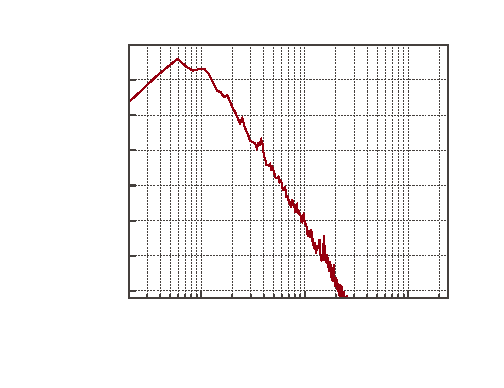
\includegraphics{Images/plot}}%
    \gplfronttext
  \end{picture}%
\endgroup

% 		\caption{LFE channel frequency spectrum}
% 	\end{figure}
% \end{frame}

% \subsection{Tables}
% \begin{frame}{Table}
% \begin{table}[]
% 	\caption{Selection of window function and their properties}
% 	\begin{tabular}[]{lrrr}
% 		\toprule
% 		\textbf{Window}			& \multicolumn{1}{c}{\textbf{First side lobe}}	
% 		                    & \multicolumn{1}{c}{\textbf{3\,dB bandwidth}}
% 		                    & \multicolumn{1}{c}{\textbf{Roll-off}} \\
% 		\midrule
% 		Rectangular				& 13.2\,dB	& 0.886\,Hz/bin	& 6\,dB/oct		\\[0.25em]
% 		Triangular				& 26.4\,dB	& 1.276\,Hz/bin	& 12\,dB/oct	\\[0.25em]
% 		Hann					& 31.0\,dB	& 1.442\,Hz/bin	& 18\,dB/oct	\\[0.25em]
% 		Hamming					& 41.0\,dB	& 1.300\,Hz/bin	& 6\,dB/oct		\\
% 		\bottomrule
% 	\end{tabular}
% 	\label{tab:WindowFunctions}
% \end{table}
% \end{frame}

% \subsection{Formulas}
% \begin{frame}{Formulas}
% \begin{block}{Fourier Integral}
% \begin{equation*}
% F(\textrm{j}\omega) = \int\limits_{-\infty}^{\infty} f(t)\cdot\textrm{e}^{-\textrm{j}\omega t} dt
% \end{equation*}
% \end{block}
% \begin{block}{Factorial}
% \begin{equation*}
% 	n! = 1\cdot 2 \cdot 3 \cdot\ldots\cdot n = \prod_{k=1}^n k
% \end{equation*}
% \end{block}
% \end{frame}

% \begin{frame}{Mindmap with TikZ}
% \centering
% % \resizebox{0.8\textheight}{!}{%
% \begin{tikzpicture}[scale=0.88]
% 	%\tikzset{every child/.append style={level distance=250}}
% 	\path[mindmap,concept color=sleekSec3Comp,text=sleekWarmGreyDark,yshift=3cm]
% 	node[concept] {\TeX}
% 	[clockwise from=-30]
% 	child[concept color=sleekSec2Dark,text=white] { node[concept] {\textcolor{white}{XeTeX}} }
% 	child[concept color=sleekSec1CompDark,text=white,yshift=0.1cm] { node[concept]{ConTex} }
% 	child[concept color=sleekSec1Dark,text=white] { node[concept] {\LaTeX} };
% \end{tikzpicture}%
% % }
% \end{frame}

% \subsection{Footnote}
% \begin{frame}{Footnotes}
% 	Lorem ipsum dolor sit amet, consetetur sadipscing elitr, sed diam nonumy eirmod tempor invidunt ut labore et dolore magna aliquyam erat, sed diam voluptua. At vero eos et accusam et justo duo dolores et ea rebum. Stet clita kasd gubergren, no sea takimata sanctus est Lorem ipsum dolor sit amet. Lorem \footnote{Lorem ipsum dolor sit amet} ipsum dolor sit amet, consetetur sadipscing elitr, sed diam nonumy eirmod tempor invidunt ut labore et dolore magna aliquyam erat, sed diam voluptua. At vero eos et accusam et justo duo dolores et ea rebum. Stet clita kasd gubergren, no sea takimata sanctus est Lorem ipsum dolor sit amet.
% \end{frame}

% \subsection{Notes}
% \begin{frame}{slide with associated notes slide}
%     This slide is for the audience.

% 	The following programmes are suitable for its presentation:
% 	\begin{itemize}
% 		\item Splitshow (Mac OS X)\\url{https://code.google.com/p/splitshow/}
% 		\item pdf-presenter (Windows)\\url{https://code.google.com/p/pdf-presenter/}
% 	\end{itemize}
% \end{frame}

% \note{
%     Use this slide for your notes on the presentation.
    
% 	The following programmes are suitable for your presentation:
% 	\begin{itemize}
% 		\item Splitshow (Mac OS X)\\\url{https://code.google.com/p/splitshow/}
% 		\item pdf-presenter (Windows)\\\url{https://code.google.com/p/pdf-presenter/}
% 	\end{itemize} 
% }

% \subsection{Columns}
% \begin{frame}{Two columns}
% 	\begin{multicols}{2}
% 		Lorem ipsum dolor sit amet, consetetur sadipscing elitr, sed diam nonumy eirmod tempor invidunt ut labore et dolore magna aliquyam erat, sed diam voluptua. At vero eos et accusam et justo duo dolores et ea rebum. Stet clita kasd gubergren, no sea takimata sanctus est Lorem ipsum dolor sit amet.
% 		\begin{itemize}
%         	\item one entry
%         	\item another entry
% 		\end{itemize}
% 	\end{multicols}
% \end{frame}

% \begin{frame}{Column break}
% 	\begin{multicols}{2}
% 		Lorem ipsum dolor sit amet, consetetur sadipscing elitr, sed diam nonumy eirmod tempor invidunt ut labore et dolore magna aliquyam erat, sed diam voluptua. At vero eos et accusam et justo duo dolores et ea rebum. Stet clita kasd gubergren, no sea takimata sanctus est Lorem ipsum dolor sit amet.
% 		\columnbreak
% 		\begin{itemize}
%         	\item one entry
%         	\item another entry
% 		\end{itemize}
% 	\end{multicols}
% \end{frame}

% \begin{frame}{References}
% 	\begin{thebibliography}{10}
    
% 	\beamertemplatebookbibitems
% 	\bibitem{Oppenheim2009}
% 	Alan~V.~Oppenheim
% 	\newblock \doublequoted{Discrete-Time Signal Processing}
% 	\newblock Prentice Hall Press, 2009

% 	\beamertemplatearticlebibitems
% 	\bibitem{EBU2011}
% 	European~Broadcasting~Union
% 	\newblock \doublequoted{Specification of the Broadcast Wave Format (BWF)}
% 	\newblock 2011
%   \end{thebibliography}
% \end{frame}

% \section{Outlook}
% \begin{frame}{To do}
% 	\begin{itemize}
% 		\item An option to a more complete footline needs to be added.
% 	\end{itemize}
% \end{frame}

% \begin{frame}{Questions, Comments, Contact}
% 	The SLEEK theme is licensed under the \quoted{GNU Public License}. So it may be redistributed and modified as long as the license type is kept.
	
% 	Please feel free to contact me if you have any questions or comments.
% 	\begin{itemize}
% 		\item \href{mailto:up201806093@up.pt}{up201806093@up.pt}
% 	\end{itemize}
% \end{frame}

\end{document}






